% 中心力场问题

\pentry{极坐标系\upref{PolA}, 二体系统\upref{TwoBD}, 角动量守恒(单个质点)\upref{AMLaw1}, 机械能守恒(单个质点)\upref{ECnst}}
\bb{中心力场问题} 可以表述为: 在惯性系中, 若一个质点只受来自某固定点的力
\begin{equation}\label{CenFrc_eq1}
\vec F(\vec r) = F(r) \uvec r
\end{equation}
求质点的运动规律.

首先注意力场 $\vec F(\vec r)$ 是一个保守场(见\autoref{Gravty_eq3}\upref{Gravty}), 所以中心力场问题也可以用势能函数 $V(r)$ 来描述(\autoref{Gravty_eq7}\upref{Gravty}), 且有
\begin{equation}
F(r) = -\dv*{V(r)}{r}
\end{equation}

我们已知二体系统\upref{TwoBD} 的运动可以等效为单个质点的中心力场问题, 所以在接下来的讨论中, 只需把质点质量 $m$ 和位矢 $\vec r$ 分别替换成约化质量 $\mu$ 和相对矢量 $\vec R$ 即可拓展到二体系统.

\subsection{极坐标中的运动方程}
由于\autoref{CenFrc_eq1} 中的 $F(r)$ 与位置矢量 $\vec r$ 的方向无关, 在极坐标系\upref{Polar} 中处理中心力场问题通常比较简单. 极坐标中质点的速度和加速度\upref{PolA} 分别为
\begin{align}
\dot{\vec r} &= \dot r \uvec r + r\dot\theta\uvec\theta\label{CenFrc_eq2}\\
\ddot{\vec r} &= (\ddot{r} - r \dot\theta^2)\uvec r + \frac 1r \dv{t} (r^2\dot\theta)\uvec \theta\label{CenFrc_eq3}
\end{align}
由\autoref{CenFrc_eq2} 得质点的角动量在极坐标中的表示为
\begin{equation}\label{CenFrc_eq4}
\vec L = \vec r \cross (m \dot{\vec r})
= mr \uvec r \cross (\dot r \uvec r + r\dot\theta \uvec\theta)
= mr^2\dot \theta \uvec z
\end{equation}
其中 $\uvec z$ 是垂直于极坐标平面的单位矢量(这个符号来自柱坐标系\upref{Cylin}). 

我们现在把\autoref{CenFrc_eq3} 代入牛顿第二定律\upref{New3} $\vec F = m\ddot{\vec r}$, 由于 $\vec F$ 只延 $\uvec r$ 方向,有 $\dv*{(r^2\dot\theta)}{t} = 0$, 即 $r^2\dot\theta$ 为常量, 代入\autoref{CenFrc_eq4} 可知质点角动量守恒. 另外在 $\uvec r$ 方向可得
\begin{equation}\label{CenFrc_eq5}
m(\ddot{r} - r \dot\theta^2) = F(r)
\end{equation}
使用\autoref{CenFrc_eq4} 消去\autoref{CenFrc_eq5} 中的 $\dot\theta$, 得
\begin{equation}\label{CenFrc_eq7}
m\ddot r = F(r) + \frac{L^2}{mr^3}
\end{equation}
该式被称为中心力场问题的\bb{径向方程}.

\subsection{一维等效势能与稳定轨道}
由于\autoref{CenFrc_eq7} 中不含 $\theta$, 我们可以将其等效为一个一维问题%粒子在一维势场 V(x) 中的运动, 未完成
, 等号右侧看做等效力 $F'(r)$. 求等效力的反原函数可得一维\bb{等效势能}
\begin{equation}
V'(r) = V(r) + \frac{L^2}{2mr^2}
\end{equation}
自然地, 我们可以利用等效一维问题中的能量守恒列出 $r(t)$ 的一阶微分方程\footnote{\autoref{CenFrc_eq9}可以在极坐标系中直接推出, 先列出 $E = m\vec v^2/2 + V(r)$, 再将\autoref{CenFrc_eq2} 代入, 并用\autoref{CenFrc_eq4} 消去 $\dot\theta$ 即可.}
\begin{equation}\label{CenFrc_eq9}
E = \frac 12 m\dot r^2 + V'(r) = \frac 12 m\dot r^2 + \frac{L^2}{2mr^2} + V(r)
\end{equation}
即
\begin{equation}
\dot r = \sqrt{\frac 2m [E - V'(r)]}
\end{equation}
这是一个可分离变量的一阶常微分方程, %链接未完成
分离变量然后两边积分得
\begin{equation}
t = \int_{r_0}^{r} \frac{\dd{r}}{\sqrt{\frac 2m [E - V'(r)]}}
\end{equation}
积分后即可逆向得到 $r(t)$.

从一维等效势能还可以判断轨道的稳定性, 我们来看一个例子

\begin{figure}[ht]
\centering
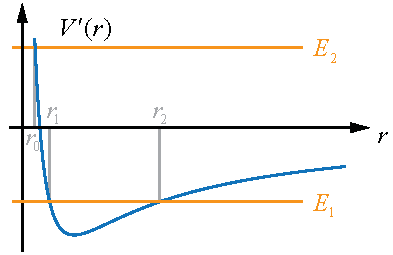
\includegraphics[width=7cm]{./figures/CenFrc1.pdf}
\caption{万有引力的一维等效势能} \label{CenFrc_fig1}
\end{figure}

\begin{exam}{万有引力}
对万有引力, $V(r) = -GMm/r$, 等效势能的大致图像如\autoref{CenFrc_fig1}.注意 $V'(r)$ 的形状还取决于常数 $L$, 但根据“用极值点确定函数图像\upref{DerImg}”, 曲线总存在一个最小值, 且 $\lim\limits_{r\to\infty}V'(r) = 0$, $\lim\limits_{r\to 0} V'(r) = +\infty$.

若质点具有能量 $E_2 > 0$, 由图可得这个质点不可能一直绕力心旋转, 而是从无穷远处入射, 在距离 $r_0$ 时开始远离力心, 最终回到无穷远. 若质点具有能量 $E_1 < 0$, 由图可知 $r$ 始终在 $[r_1, r_2]$ 区间内往返变动(在“开普勒问题\upref{CelBd}”中, 我们将会知道 $E_1$ 和 $E_2$ 分别对应椭圆轨道和双曲线轨道). 特殊地, 当质点能量等于 $V'(r)$ 的最小值时, 它与力心的距离将保持不变, 即轨道为圆形. 若给处于圆形轨道的质点一个扰动, $r$ 将在曲线最低点附近振动, 且振动频率由最低点处曲线的二阶导数决定%链接未完成, 链接到一维势能的应用
, 我们将这种不会因为扰动而彻底改变的轨道叫做\bb{稳定}轨道.
\end{exam}

\begin{figure}[ht]
\centering
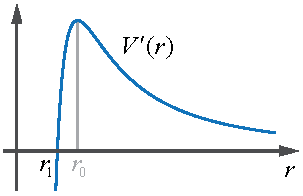
\includegraphics[width=5.7cm]{./figures/CenFrc2.pdf}
\caption{四次方反比力的一维等效势能} \label{CenFrc_fig2}
\end{figure}

\begin{exam}{四次方反比力}
作为一个不稳定轨道的例子, 我们来考察 $V(r) = -k/r^3$, 其中 $k$ 是一个大于零的常数. 等效势能的大致图像如\autoref{CenFrc_fig2}. 若质点的能量大于 $V'(r_0)$, 则质点会从无穷远入射, 穿过力心然后回到无穷远, 若质点的能量小于零, 它将被困在 $r < r_1$ 的圆形势阱内并不断穿过力心. 若质点的能量恰好为 $V'(r_0)$, 那么它将以 $r_0$ 为半径做圆周运动, 然而任何微小的扰动都会使其从势能曲线顶端向两侧滑落, 从而彻底改变轨道的性质. 我们说这样的轨道是\bb{不稳定}的.
\end{exam}

